\documentclass[11pt]{article}

\usepackage[margin=1in]{geometry}
\usepackage{graphicx}
\usepackage{amsmath,amssymb,amsfonts}
\usepackage{booktabs}
\usepackage{siunitx}
\usepackage{float}

\raggedbottom

\begin{document}

\title{Supplementary Information: The wind is always blowing somewhere in Europe}
\author{}
\date{}

\maketitle

This Supplementary Information accompanies the main manuscript ``The wind is always blowing somewhere in Europe: A decade of evidence for continental-scale renewable baseload.''


%%=============================================================%%
%% Supplementary Figures
%%=============================================================%%

\section*{Supplementary Figures}

\begin{figure}[H]
    \centering
    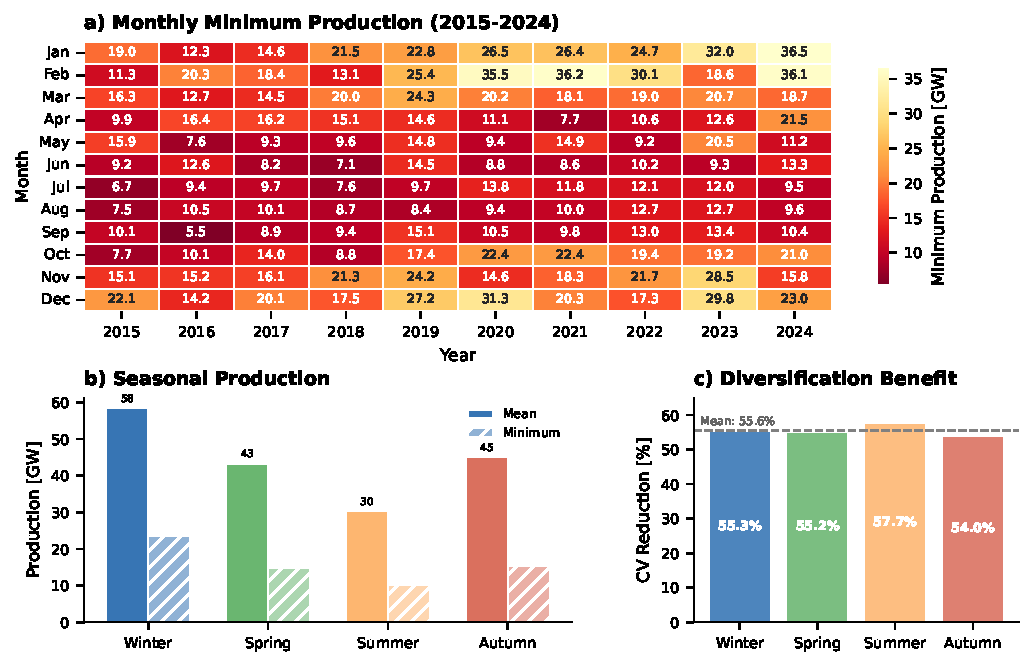
\includegraphics[width=\textwidth]{Figures_Paper/figure3_seasonal.pdf}
    \caption{\textbf{Supplementary Figure 1: Seasonal structure of European wind production (2015--2024).} \textbf{a,} Monthly minimum production heatmap showing higher winter minimums (typically 15--36~GW) and lower summer minimums (7--14~GW), reflecting seasonal wind patterns. \textbf{b,} Seasonal mean and minimum production: winter leads with 58~GW mean and 23~GW minimum, while summer has the lowest mean (30~GW) and minimum (10~GW). \textbf{c,} Seasonal diversification benefit (DB): summer provides the strongest diversification (DB~$= 57.7\%$), consistent with localized thermal wind patterns that are less correlated across countries than winter's synoptic-scale systems.}
    \label{fig:seasonal}
\end{figure}

\begin{figure}[H]
    \centering
    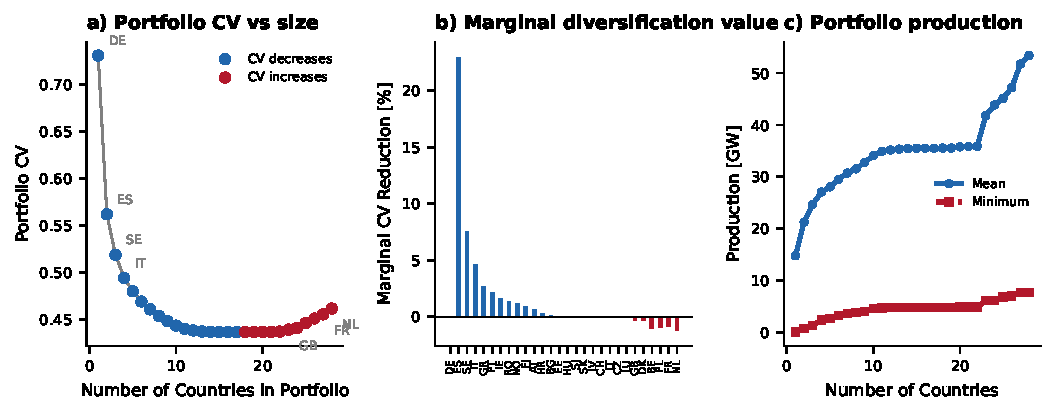
\includegraphics[width=\textwidth]{Figures_Paper/figure_marginal_diversification.pdf}
    \caption{\textbf{Supplementary Figure 2: Marginal diversification curves.} Greedy portfolio construction described in the main text (Table~2). Starting from Germany (CV = 0.73), each successive country is added to minimize portfolio CV. \textbf{a,} Portfolio CV versus number of countries: blue points indicate beneficial additions, red points indicate countries that \textit{increase} CV. The minimum CV (0.437) is reached at 17 countries; subsequent additions---GB, DK, BE, PL, FR, NL---increase CV because they are tightly correlated with the existing portfolio. \textbf{b,} Marginal CV reduction per country: the first five (Spain, Sweden, Italy, Greece, Portugal) contribute the majority of the total CV reduction. \textbf{c,} Portfolio mean and minimum production grow monotonically as countries are added.}
    \label{fig:marginal}
\end{figure}

\begin{figure}[H]
    \centering
    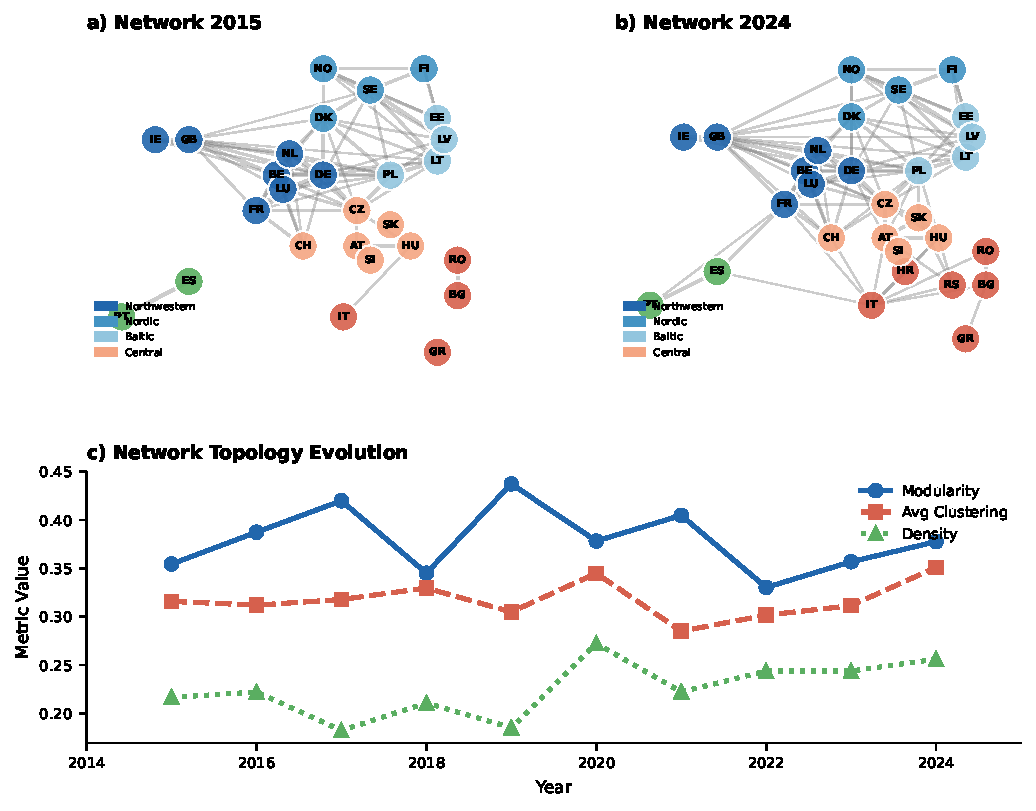
\includegraphics[width=\textwidth]{Figures_Paper/figure_network_evolution.pdf}
    \caption{\textbf{Supplementary Figure 3: Evolution of the wind correlation network (2015--2024).} Annual correlation networks with countries as nodes and edges for pairs with $|r| > 0.3$. Network density increased from 0.22 (2015) to 0.26 (2024), indicating growing spatial correlation. The number of Louvain communities decreased from 8 to 4, consistent with consolidation into fewer, larger clusters driven by North Sea offshore expansion and capacity concentration in Northwestern Europe.}
    \label{fig:network}
\end{figure}



\begin{figure}[H]
    \centering
    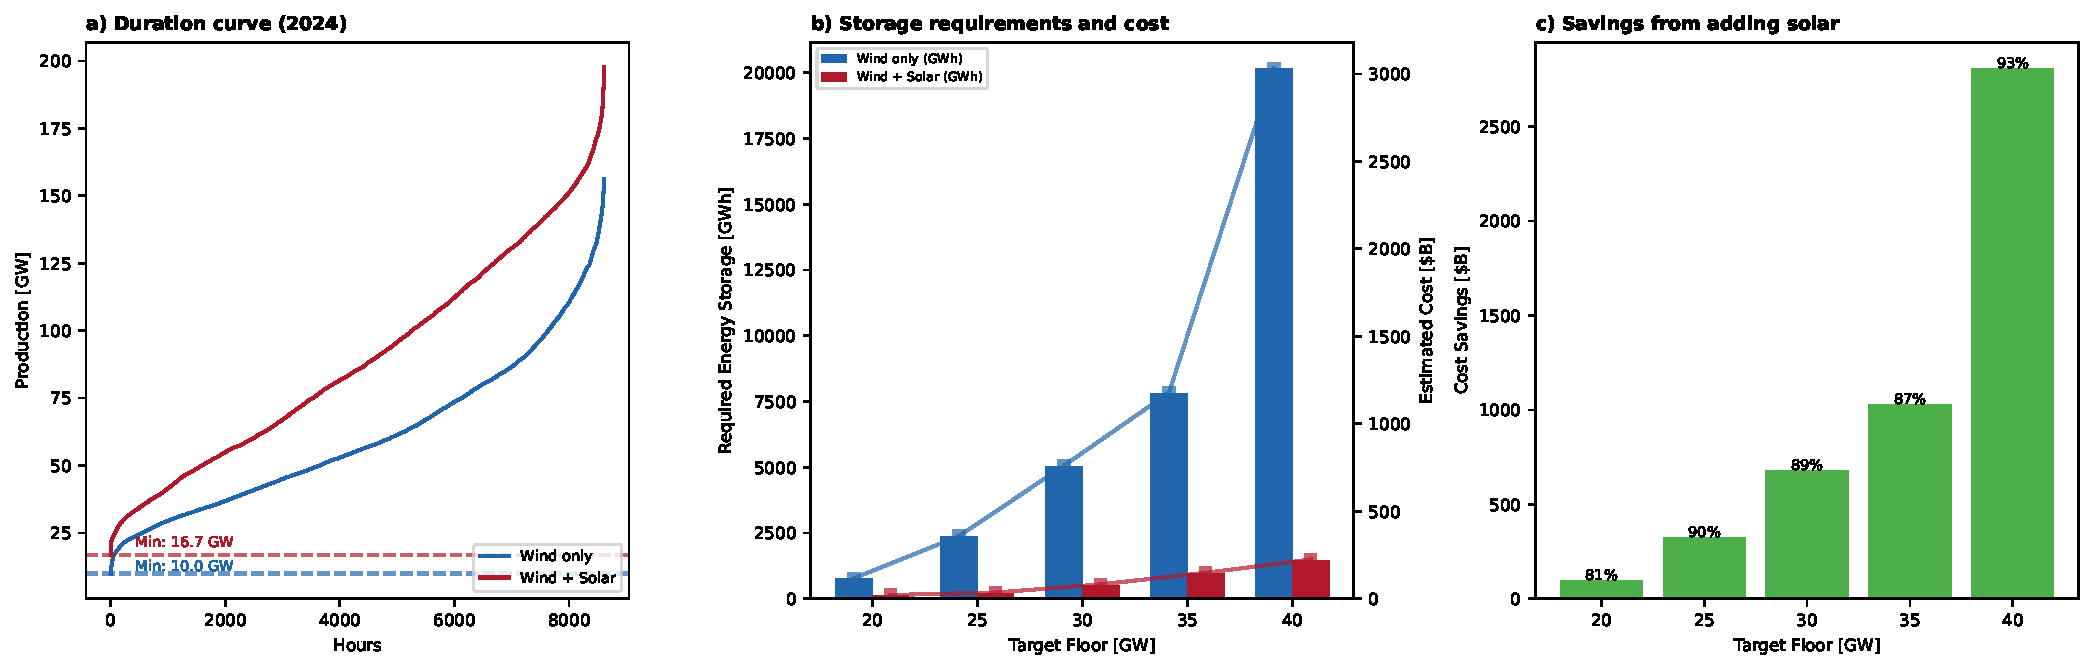
\includegraphics[width=\textwidth]{Figures_Paper/figure_battery_storage.pdf}
    \caption{\textbf{Supplementary Figure 4: Battery storage requirements---wind-only vs combined wind+solar.} \textbf{a,} Duration curves for 2024 showing combined wind+solar achieves higher minimum production (wind-only minimum: 10.0~GW; combined: 16.7~GW without any storage). \textbf{b,} Energy storage requirements (bars, left axis) and estimated cost (lines, right axis) for different guaranteed floor levels, comparing wind-only and combined wind+solar portfolios. \textbf{c,} Absolute cost savings from using the combined portfolio, with percentage savings (81--93\%) labelled.}
    \label{fig:battery}
\end{figure}

\begin{figure}[H]
    \centering
    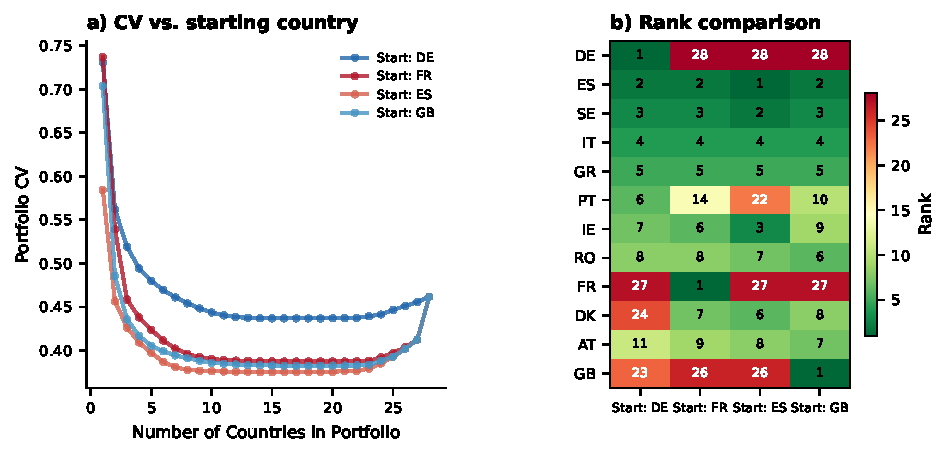
\includegraphics[width=\textwidth]{Figures_Paper/figure_sensitivity_start_country.pdf}
    \caption{\textbf{Supplementary Figure 5: Sensitivity of greedy portfolio construction to starting country.} \textbf{a,} Portfolio CV as a function of countries added, starting from four different anchor countries (Germany, France, Spain, Great Britain). All curves converge to the same final CV ($\sim$0.46) by $\sim$15 countries, and the first five additions produce $>$90\% of the total benefit regardless of starting point. \textbf{b,} Rank heatmap showing the order in which countries are added for each starting country. The top diversifiers---Spain, Sweden, Italy, Greece---consistently appear in the top five (dark green), while the starting country's own cluster members (e.g., France and Great Britain when starting from Germany) are added last (red), confirming that within-cluster correlation limits their marginal value.}
    \label{fig:sensitivity}
\end{figure}

\section*{Supplementary Tables}

\begin{table}[H]
\centering
\caption{\textbf{Supplementary Table 1: Battery storage requirements---wind-only vs combined wind+solar.} Storage energy (GWh), cost (\$B at \$150/kWh + \$200/kW, a lower-bound estimate; see Methods), and percentage savings for five guaranteed floor targets. Percentage savings are robust to cost assumptions (shifting by $<$2 percentage points at \$300/kWh). Costs assume 100\% coverage over the decade (worst case); real deployments targeting 99.9\% reliability would need substantially less.}
\label{tab:battery}
\begin{tabular}{S[table-format=2.0]S[table-format=5.0]S[table-format=4.0]S[table-format=4.0]S[table-format=3.0]S[table-format=2.0]}
\toprule
& \multicolumn{2}{c}{Energy [GWh]} & \multicolumn{2}{c}{Cost [\$B]} & \\
\cmidrule(lr){2-3} \cmidrule(lr){4-5}
{Floor [GW]} & {Wind} & {W+S} & {Wind} & {W+S} & {Savings [\%]} \\
\midrule
20 & 760 & 130 & 117 & 22 & 81 \\
25 & 2358 & 215 & 358 & 36 & 90 \\
30 & 5037 & 521 & 761 & 83 & 89 \\
35 & 7807 & 957 & 1177 & 149 & 87 \\
40 & 20156 & 1453 & 3030 & 224 & 93 \\
\bottomrule
\end{tabular}
\end{table}

\begin{table}[H]
\centering
\caption{\textbf{Supplementary Table 2: Annual baseload comparison---wind-only vs combined wind+solar.} Minimum hourly production (GW) for wind-only and combined wind+solar portfolios, with the baseload improvement factor and aggregate wind-solar Pearson correlation. Wind minimums here are computed on hours common to both wind and solar datasets; values may differ slightly from Table~1 in the main text, which uses all available wind hours. The number of solar countries grows over the decade as ENTSO-E reporting expanded.}
\label{tab:combined_baseload}
\begin{tabular}{l S[table-format=2.0] S[table-format=2.0] S[table-format=2.1] S[table-format=2.1] S[table-format=3.0] S[table-format=2.2, retain-explicit-plus]}
\toprule
& \multicolumn{2}{c}{Countries} & \multicolumn{2}{c}{Min.\ production [GW]} & & \\
\cmidrule(lr){2-3} \cmidrule(lr){4-5}
{Year} & {Wind} & {Solar} & {Wind} & {W+S} & {Impr.\ [\%]} & {$r_{\text{W--S}}$} \\
\midrule
2015 & 27 & 20 & 6.7 & 9.0 & 34 & -0.21 \\
2016 & 27 & 19 & 5.5 & 8.7 & 60 & -0.21 \\
2017 & 27 & 19 & 8.2 & 9.1 & 11 & -0.20 \\
2018 & 27 & 19 & 7.1 & 11.4 & 61 & -0.28 \\
2019 & 28 & 20 & 8.4 & 12.9 & 54 & -0.26 \\
2020 & 28 & 21 & 8.8 & 12.9 & 46 & -0.25 \\
2021 & 28 & 22 & 7.7 & 15.9 & 106 & -0.23 \\
2022 & 29 & 23 & 10.2 & 17.5 & 71 & -0.28 \\
2023 & 29 & 24 & 9.9 & 20.2 & 104 & -0.32 \\
2024 & 29 & 25 & 10.0 & 16.7 & 67 & -0.33 \\
\midrule
\multicolumn{3}{l}{Decade average} & 8.3 & 13.4 & 61 & -0.26 \\
\bottomrule
\end{tabular}
\end{table}


\begin{table}[H]
\centering
\caption{\textbf{Supplementary Table 3: Top-10 country ranking comparison across starting countries.} Each column shows the rank at which the country is added to the greedy portfolio when starting from a different anchor country. The top diversifiers (Spain, Sweden, Italy) maintain their position in the top five regardless of starting point, confirming that the main-text ranking (Table~2, starting from Germany) is robust. Minor rank swaps occur among countries with similar marginal contributions (e.g., Greece and Portugal may exchange positions), but the core finding---that Iberian, Nordic, and Southern European countries dominate the diversification value---is insensitive to starting country choice.}
\label{tab:sensitivity}
\begin{tabular}{llllll}
\toprule
Rank & Start: DE & Start: FR & Start: ES & Start: GB \\
\midrule
1 & DE & FR & ES & GB \\
2 & ES & ES & SE & ES \\
3 & SE & SE & IE & SE \\
4 & IT & IT & IT & IT \\
5 & GR & GR & GR & GR \\
6 & PT & IE & DK & RO \\
7 & IE & DK & RO & AT \\
8 & RO & RO & AT & DK \\
9 & NO & AT & NO & IE \\
10 & FI & NO & BG & PT \\
\midrule
\multicolumn{5}{l}{Final CV (all start countries): 0.462} \\
\bottomrule
\end{tabular}
\end{table}

\begin{table}[H]
\centering
\caption{\textbf{Supplementary Table 4: Three formulations of the diversification benefit (DB).} The \textit{unweighted} DB (Eq.~1 in the main text) treats each country equally; the \textit{production-weighted} DB weights each country's CV by its share of total production; the \textit{CF-normalized} DB replaces raw production with capacity factors ($\bar{P}/P_{\text{installed}}$), removing the mechanical effect of capacity growth. Production weighting reduces DB to $\sim$38\% because large producers (Germany, France) are more correlated with the aggregate than small, peripheral countries. All three variants are stable across the decade, confirming that the diversification benefit is a property of European wind climatology, not an artifact of weighting or capacity expansion.}
\label{tab:cf_comparison}
\begin{tabular}{l S[table-format=2.1] S[table-format=2.1] S[table-format=2.1]}
\toprule
 & \multicolumn{3}{c}{DB [\%]} \\
\cmidrule(lr){2-4}
{Year} & {Unweighted} & {Prod.-Weighted} & {CF-Normalized} \\
\midrule
2015 & 51.1 & 42.3 & 48.3 \\
2016 & 51.8 & 42.3 & 49.4 \\
2017 & 47.3 & 39.1 & 45.7 \\
2018 & 44.0 & 36.0 & 44.1 \\
2019 & 57.0 & 39.3 & 47.0 \\
2020 & 44.5 & 35.3 & 42.5 \\
2021 & 45.7 & 37.0 & 43.5 \\
2022 & 48.1 & 36.7 & 45.9 \\
2023 & 45.0 & 37.4 & 43.2 \\
2024 & 43.5 & 35.7 & 42.7 \\
\midrule
\multicolumn{1}{l}{Mean} & 47.8 & 38.1 & 45.2 \\
\bottomrule
\end{tabular}
\end{table}


\end{document}
